%---------- Segundo Capitulo ----------
\chapter{Metodologia}
\label{chap:desen}

Nesta seção será apresentado o desenvolvimento de todo o projeto, na ordem que o mesmo foi criado. Desta forma fica mais fácil para o leitor entender o desenvolvimento do projeto, além de poder ser utilizado como base para projetos futuros mais facilmente.

\section{Construção do Tacômetro Digital}
Um tacômetro não é nada mais que um frequencímetro modificado. Enquanto este mede a frequência de uma onda, aquele é capaz de medir a frequência de um objeto (desde que este objeto realize rotações).

A forma mais fácil de se construir tal ferramenta é utilizando dois LED's infravermelhos, um receptor e outro emissor. Inicialmente, a conexão entre os dois está alta (ativa), e quando esta conexão se torna baixa (inativa) significa que algo cortou o sinal entre os dois LED's. Desta forma, podemos desenvolver um algoritmo para contar quantas vezes este sinal é cortado em um minuto, podendo determinar a frequência do motor utilizado no projeto.

O diagrama esquemático deste projeto é simples, e será apresentado na figura 3.

\begin{figure}[!h]
	\centering
	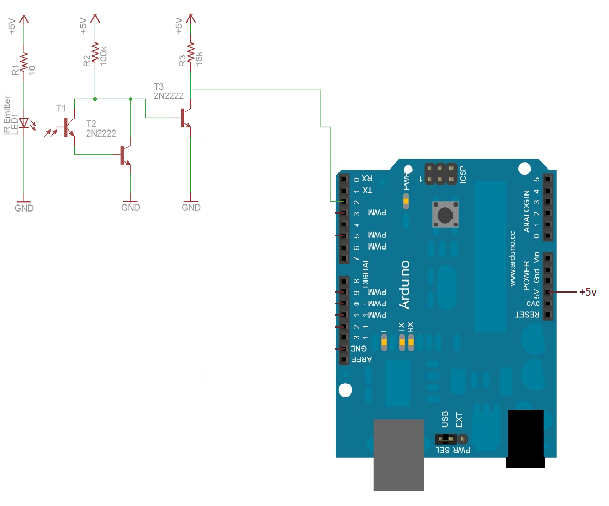
\includegraphics{./tachometer_schematic.png}
	\caption[Diagrama Esquemático do Tacômetro Digital]{Diagrama Esquemático do Tacômetro Digital}
	\label{fig:tachometer_diagram}
\end{figure}

Um cuidado especial que teve que ser tomado é a posição dos LED's. É importante que estes estejam a uma certa distância um do outro, mas não muito afastados, e também perfeitamente alinhados, para que o sinal recebido pelo LED receptor seja alto o suficiente para manter todo o sistema em alto, enquanto o motor não cortá-lo. Uma distância razoável é mostrada na figura 4.

\begin{figure}[!h]
	\centering
	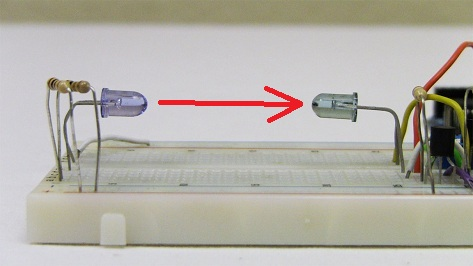
\includegraphics{./break__beam_small.jpg}
	\caption[Distância razoável para os LED's]{Distância razoável para os LED's}
	\label{fig:break__beam_small}
\end{figure}

Com o hardware feito, foi necessário desenvolver um algoritmo para a contagem da frequência. Vale lembrar que o próprio Arduino possui diversas bibliotecas e funções que facilitaram o desenvolvimento do nosso algoritmo. A função attachInterrupt(), por exemplo, é chamada no momento que uma interrupção no sistema existe~\cite{Arduino_attachInterrupt()}.

\begin{lstlisting}
volatile float time = 0;
volatile float time_last = 0;
volatile int rpm_array[5] = {0,0,0,0,0};

void setup()
{
  //Pino Digital 2 foi definido como interruptor
 attachInterrupt(0, fan_interrupt, FALLING);

  // Mensagem no prompt de comando do Arduino
  Serial.print("Current RPM:");
}

//Funcao Loop que calcula a RPM do motor e atualiza
//este valor na saida Serial
void loop()
{
    int rpm = 0;

    while(1)
    {
        //Define a velocidade de atualizacao da contagem
        delay(400);

        Serial.print("                ");

        //Atualiza a contagem do RPM
        Serial.print(rpm);

        //Atualiza o RPM
        if(time > 0)
        {
            //Para obtermos um valor mais proximo do real, utili-
            //zaremos uma media entre 5 medicoes consecutivas
            rpm_array[0] = rpm_array[1];
            rpm_array[1] = rpm_array[2];
            rpm_array[2] = rpm_array[3];
            rpm_array[3] = rpm_array[4];

            //4 e o numero de helices do motor
            rpm_array[4] = 60*(1000000/(time*4));

            rpm = (rpm_array[0] + rpm_array[1] + rpm_array[2]
            + rpm_array[3] + rpm_array[4]) / 5;
        }
    }
}

//Ponto que o sinal entre os dois LED's e cortado pelo motor
void fan_interrupt()
{
   time = (micros() - time_last);
   time_last = micros();
}
\end{lstlisting}

Com isto, foi possível determinar a velocidade do motor de 2400 rpm ou uma frequência de 40 Hz.

\section{Construção do Motor}
Um ponto chave no desenvolvimento do projeto foi encontrar uma solução para girar a PCI com uma velocidade suficiente para gerar o efeito de persistência da visão com uma resolução que fosse agradável aos olhos.
Para tal, escolhemos utilizar coolers de gabinete de computador. Em um primeiro momento testamos um cooler pequeno, com alimentação de 12 V. Ele girava a placa (uma protoboard, em uma fase bem primitiva dos testes) com uma velocidade muito abaixo do esperado. Além disse foi necessário quebrar a parte plástica que cobria o cooler para podermos conectar a placa à peça central giratória.
Como a velocidade deste cooler não foi suficiente, pesquisamos e compramos um cooler com alimentação de 127~230V, da marca Ultrar. Este cooler é mostrado na figura 5.

\begin{figure}[!h]
	\centering
	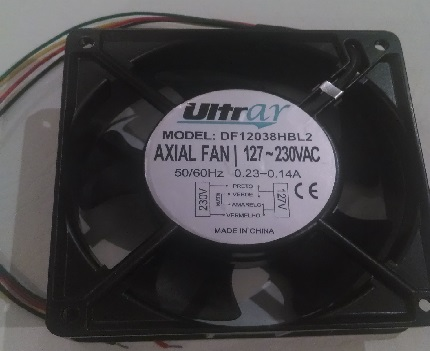
\includegraphics{./cooler1.jpg}
	\caption[Cooler utilizado no projeto final]{Cooler utilizado no projeto final}
	\label{fig:cooler_Ultrar}
\end{figure}


Utilizamos 127V, e a velocidade de rotação atingiu o nível que tínhamos em mente. Porém, com este cooler mais potente, o problema de conectar a placa na parte giratória era mais difícil de ser resolvido pois, ao contrário do cooler de 12V que era revestido por plástico, esse cooler é revestido por uma placa de metal maciço. Como esse cooler gira tão rápido que chega a ser perigoso para quem o está manejando, decidimos manter essa peça de metal e criar uma solução para conseguir manter a protoboard fixa à peça giratória. Era necessário elevar a placa aproximadamente 15 mm da peça giratória. Isso se dá ao fato de que a proteção é um pouco mais alta que a peça giratória, e isso causaria atrito entre a placa e a proteção. Esta proteção é mostrada na figura 6.

\begin{figure}[!h]
	\centering
	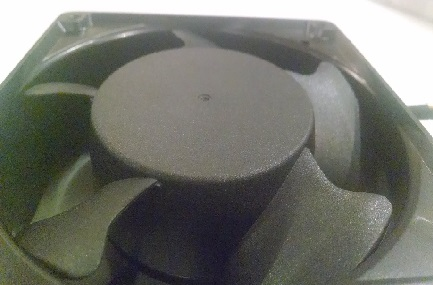
\includegraphics{./cooler2.jpg}
	\caption[Proteção do cooler]{Proteção do cooler}
	\label{fig:cooler_protecao}
\end{figure}

Em um primeiro momento, foi decidido soldar a bateria que alimenta o Arduino na própria placa de LEDs e depois criar um contrapeso para que não ficasse instável. Como a bateria cabe dentro da parte redonda do cooler, ao colocá-la ali conseguimos resolver dois problemas: o do contrapeso da placa e o da elevação em relação à proteção. Portanto a bateria foi fixada em cima da parte central do cooler e a placa em cima da bateria.

\section{Construção da PCI}
A  parte eletrônica do projeto envolvia criar uma placa onde todos os 17 LEDs estivessem conectados ao Arduino e funcionando.

Primeiramente, é importante mostrar o esquemático, utilizado como base para o desenvolvimento da placa. Este esquemático é apresentado na figura 7.

\begin{figure}[!h]
	\centering
	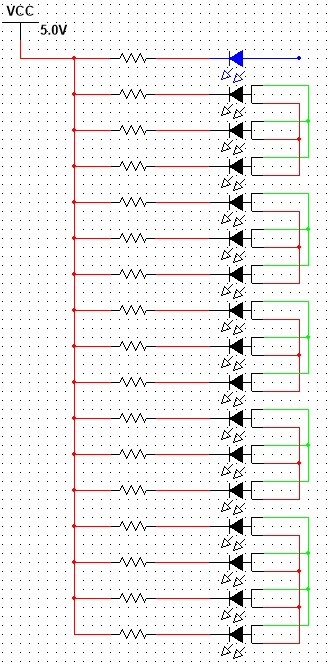
\includegraphics{./esquematico.jpg}
	\caption[Esquemático base para a solda]{Esquemático base para a solda}
	\label{fig:esquematico}
\end{figure}

Em um primeiro momento utilizamos uma protoboard para montar protótipos, porém rapidamente vimos como esta era uma solução inadequada devido ao peso e espessura de tal componente. Então utilizamos uma matriz de contatos para posicionar os LEDs, resistores e Arduino. Isso nos dava maior flexibilidade com o posicionamento das peças além de ser muito leve e ter espessura desprezível.

Como mencionado anteriormente, a bateria foi posicionada diretamente no cooler, portanto não houve necessidade de nos preocuparmos com contrapeso. Já os LEDs foram posicionados alinhados, com resistores à esquerda e o Arduino abaixo, como apresentado na figura 8.

\begin{figure}[!h]
	\centering
	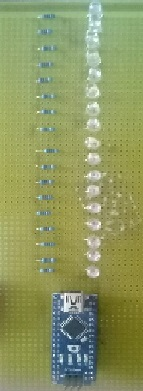
\includegraphics{./placa_cima.jpg}
	\caption[Estado final da Matriz de Contatos]{Estado final da Matriz de Contatos}
	\label{fig:placa_cima}
\end{figure}

A solda final da matriz de contatos ficou como mostrada na figura 9.

\begin{figure}[!h]
	\centering
	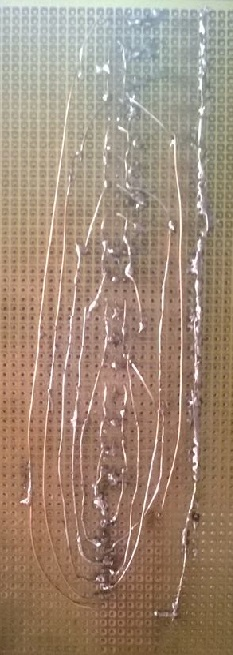
\includegraphics{./placa_baixo.jpg}
	\caption[Solda da Matriz de Contatos]{Solda da Matriz de Contatos}
	\label{fig:placa_cima}
\end{figure}

Após a finalização da solda, foi verificado que, se a a matriz de contatos fosse realmente utilizada, correríamos o risco de algum ponto de solda se soltar, ou até mesmo ocorrer um curto-circuito no sistema. Desta forma, decidimos descartar a matriz de contatos e desenvolver uma PCI. Os resultados finais serão vistos nas figuras 10 e 11.

\begin{figure}[!h]
	\centering
	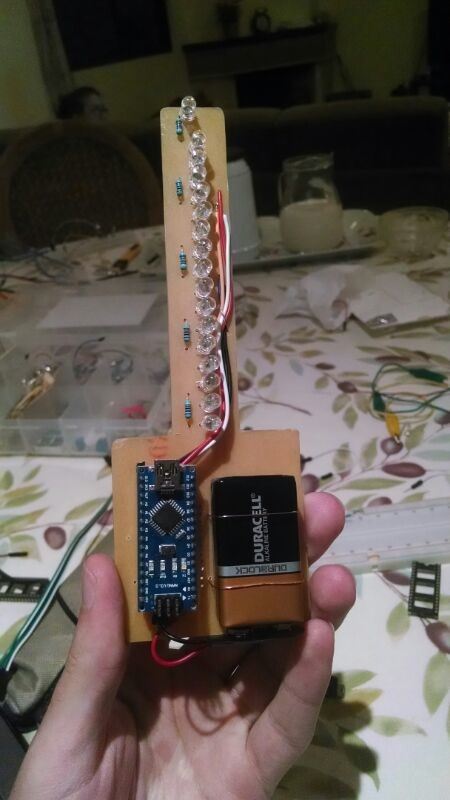
\includegraphics{./PCI_cima.jpg}
	\caption[PCI vista de cima]{PCI vista de cima}
	\label{fig:pci_cima}
\end{figure}

\begin{figure}[!h]
	\centering
	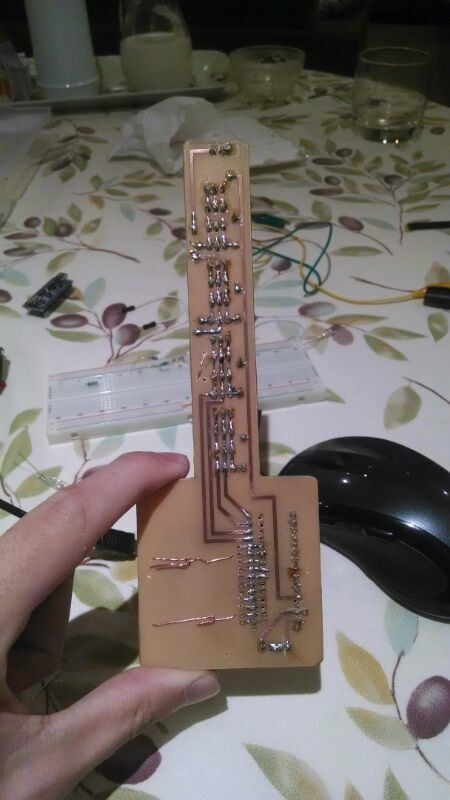
\includegraphics{./PCI_baixo.jpg}
	\caption[PCI vista de baixo]{PCI vista de baixo}
	\label{fig:pci_baixo}
\end{figure}

Vale ressaltar que, com o desenvolvimento da PCI, a bateria também mudou de lugar, para facilitar o carregamento ou até mesmo uma troca desta, caso haja necessidade.

Com a PCI criada, pudemos começar a nos preocupar com o controle dos LED's por parte do Arduino, tendo em vista o baixo número de portas deste e o alto número de LED's do relógio.
Como a velocidade de rotação varia com a distância relativa ao ponto que gira, era necessário controlar os LEDs separadamente. Se todos piscassem ao mesmo tempo haveria uma diferença perceptível e os ponteiros do relógio ficariam destorcidos. Para resolver esse problema dividimos os LEDs em 6 grupos.
O primeiro LED era controlado individualmente e ligado apenas à uma porta do Arduino. Este LED é o que gera os pontos fixos que marcam os minutos do relógio.
Os outros 16 LEDs foram divididos em 4 grupos de 3 e um de 4 LEDs cada.

Essa proporção foi escolhida pois era necessário reservar duas porta do Arduino para cada grupo, e esta limitação foi o que nos levou a dividí-los desta maneira.

Todos os grupos possuem ligações à duas portas independentes do Arduino: uma para o ponteiro dos minutos e uma para o ponteiro das horas. Isso permite que eles tenham cores distintas e também diferentes da cor do primeiro LED que indica os pontos fixos dos minutos.

Portanto o primeiro LED estava conectado à uma porta e cada um dos 5 grupos restantes estava conectado à duas, utilizando 11 portas no total.

O ponteiro dos segundos não fez parte do projeto devido ao número limitado de portas do Arduino.

A parte mais complicada desta etapa do projeto foi soldar os componentes na PCI (e na matriz de contatos). Ficou decidido que a própria equipe realizaria a solda (como forma de aprendizado), mesmo sabendo que esta não ficaria com uma qualidade ótima.

A grande dificuidade desta etapa se deu ao fato de a PCI desenvolvida (e a matriz de contatos também, mesmo que esta tenha sido descartada), possui um espaço muito limitado para cada trecho de solda, e também por possuirmos equipamentos inapropriados para a execução da mesma (Ferro de Solda de 60W, ao contrário do recomendado, que é 30W).

\section{Software}

O objetivo do algoritmo era controlar os grupos de LED de maneira que piscassem a cada volta, no lugar onde o ponteiro das horas ou minutos correspondentes devesse estar. Por exemplo, para mostrar 15:30, era necessário que os LEDs piscassem em 270$^\circ$ e 0$^\circ$ (tendo como 0 o lado direito do eixo horizontal que corta o cooler ao meio, como um círculo unitário. O cooler gira em sentido anti-horário). Ao piscar em 270$^\circ$ os LEDs mostram o ponteiro dos minutos em 30min e em 0$^\circ$ em 15h.

A ideia do algoritmos foi inspirada em relógios de pulso tradicionais. Ao invés de calcular o tempo e imprimir os minutos e horas correspondentes, um relógio tradicional é definido em um determinado horário e simplesmente incrementa os minutos e horas a partir disso.

Tendo como medida base de tempo o tempo necessário para uma volta da placa, pudemos calcular após quanto tempo depois de passar pelo ponto mais baixo cada LED deveria acender. Isso foi calculado com base no ângulo necessário para imprimir cada hora ou minuto. Dividimos o relógio em 60 subdivisões de 6$^\circ$ cada para os minutos e 12 de 30$^\circ$ para as horas. Portanto após um minuto era necessário que o LED piscasse 6$^\circ$ após o ponto onde ele havia acabado de acender. Como sabemos quanto tempo a placa demora para percorrer 360$^\circ$, podemos calcular quanto ela demora para percorrer 6$^\circ$ (Calculamos considerando uma velocidade constante, o que é apenas uma aproximação considerando que um objeto com peso distribuído de forma não uniforme, sob força da gravidade, rotacionado por um motor comprado em uma loja de rua nunca girará com velocidade constante. A aproximação se mostrou válida e não afetou os resultados). Ao voltar ao início, a contagem é redefinida. Isso permite que contemos o tempo sem precisar saber qual a hora atual. Apenas começando com a hora correta já é suficiente para que o relógio funcione. Essa ideia de incrementar ao invés de calcular é possibilitada por engrenagens em relógio; no nosso caso é possibilitada por métodos delay() e um pouco de física básica.

O primeiro LED é o mais simples, pois apenas precisa piscar a cada 6$^\circ$. Os outros grupos executam a mesma função com os mesmos loops, porém com parâmetros de delay diferentes. Estes diferentes parâmetros foram definidos com base na frequência de giro do motor e a velocidade de resposta do Arduino.

Todas as portas do Arduino foram definidas como Output e geram 0V de tensão quando ativadas, assim acendendo o LED, ou 5V, apagando-o.

O código foi desenvolvido em Processing, porém com toda a base em C. Os maiores desafios encontrados pela equipe foram os tempos de acendimento (por quanto tempo um LED deve ficar aceso), o tempo de execução dos comandos enquanto a placa gira e também a coordenação dos LEDs. Todo o código está apresentado no Anexo A.